\documentclass[conference]{IEEEtran}
\IEEEoverridecommandlockouts

\usepackage{cite}
\usepackage{amsmath,amssymb,amsfonts}
\usepackage{algorithmic}
\usepackage{graphicx}
\usepackage{textcomp}
\usepackage{xcolor}
\usepackage{hyperref}
\usepackage{listings}
\usepackage{algorithm}
\usepackage{algorithmic}
\usepackage{tikz}
\usetikzlibrary{shapes,arrows,positioning,automata}

\def\BibTeX{{\rm B\kern-.05em{\sc i\kern-.025em b}\kern-.08em
T\kern-.1667em\lower.7ex\hbox{E}\kern-.125emX}}

\begin{document}

\title{ScholarMate: An Offline-First Cross-Platform AI Research Workspace with Real-Time Collaboration and Intelligent Document Management}

\author{
\IEEEauthorblockN{Rayed Riasat Rabbi, Jawadul Karim Tanzim, Barshon Basak, Mezbah Uddin Ahmed}
\IEEEauthorblockA{
\textit{Department of Electrical and Computer Engineering (ECE)} \\
\textit{North South University} \\
Plot \#15, Block \#B, Bashundhara \\
Dhaka--1229, Bangladesh \\
rayed.rabbi@northsouth.edu, jawadul.tanzim@northsouth.edu, barshon.basak@northsouth.edu, mezbah.ahmed@northsouth.edu
}
}

\maketitle

\begin{abstract}
Modern academic research demands sophisticated document management systems that balance data ownership, offline capability, collaborative features, and AI-powered analysis. This paper presents ScholarMate, a comprehensive offline-first research workspace that addresses critical limitations in existing solutions through a hybrid Flutter-FastAPI architecture. The system enables researchers to manage PDF libraries with AI-powered semantic search, real-time collaboration, and robust annotation features while maintaining complete data ownership via Google Drive integration. Key innovations include a namespace-based vector isolation strategy for multi-tenant RAG systems, a NotebookLM-inspired study workspace with automated content generation, integrated document scanning with OCR, automated bibliography generation, and per-file real-time chat. The architecture employs local SQLite caching with Drift for offline-first operations and Supabase Realtime for collaboration. Our implementation achieves cross-platform deployment across platforms (Android, Web, Windows) from a single codebase while operating entirely on free-tier services. Performance evaluation demonstrates sub-second query response times (1.25s average), efficient memory utilization through batch processing, and seamless offline-online synchronization. The system successfully addresses vendor lock-in, high subscription costs, and limited offline capability that plague current solutions, providing a cost-free, privacy-preserving alternative for individual researchers and institutions.
\end{abstract}

\begin{IEEEkeywords}
offline-first architecture, cross-platform development, retrieval-augmented generation, real-time collaboration, document management, semantic search, Flutter, vector databases, hybrid embedding systems
\end{IEEEkeywords}

\section{Introduction}

The exponential growth of digital academic literature has created unprecedented challenges for researchers managing document collections. Current solutions such as Mendeley \cite{b1}, Zotero \cite{b2}, and commercial platforms suffer from critical limitations: vendor lock-in through proprietary storage, limited offline functionality, prohibitive subscription costs, and inadequate support for collaborative annotation workflows. These constraints particularly impact researchers in developing regions and institutions with limited budgets.


ScholarMate addresses these challenges through a novel architecture combining offline-first principles with cloud-based AI capabilities. The system stores all user documents in personal Google Drive accounts, provides optical character recognition (OCR) for scanned documents, text-to-speech functionality, semantic search using retrieval-augmented generation (RAG), collaborative annotations with conflict resolution, and a dedicated Notebook Studio for research synthesis.

The key contributions of this work include:

\begin{itemize}
\item A hybrid offline-first architecture enabling full functionality without internet connectivity while seamlessly synchronizing when online, implemented through Drift SQLite with operation queuing
\item A namespace-based vector isolation strategy for multi-tenant RAG systems using shared Pinecone infrastructure, achieving O(1) user isolation without per-user index overhead
\item Cross-platform deployment achieving feature parity across six platforms from a single Flutter codebase with platform-specific capability detection
\item Real-time collaboration system with WebSocket-based synchronization, last-write-wins conflict resolution, and per-file chat threads
\item Notebook Studio workspace inspired by NotebookLM, enabling document organization, context-aware AI chat, and automated generation of study aids (quizzes, flashcards, summaries, mind maps)
\item Integrated document scanner with on-device preprocessing and hybrid OCR pipeline (Tesseract for offline, API for online)
\item Automated citation generator supporting DOI, arXiv, ISBN, and PubMed identifiers with multiple format outputs (APA, MLA, Chicago, BibTeX)
\item Complete implementation using free-tier services (Supabase, Pinecone, GROQ), eliminating cost barriers for individual researchers
\end{itemize}


\section{Related Work}

\subsection{Document Management Systems}

Traditional reference management systems like Mendeley \cite{b1} and Zotero \cite{b2} provide citation management and basic PDF annotation but lack offline-first architecture and AI-powered semantic search. Mendeley requires constant internet connectivity and stores documents on proprietary servers, creating vendor lock-in. Zotero offers better data portability but provides limited collaboration features and no semantic search capabilities.

Cloud-based note-taking platforms such as Notion and Evernote offer collaboration features but require persistent internet connectivity and store data on proprietary infrastructure. These platforms lack specialized features for academic research such as citation management, PDF annotation, and semantic search over document collections.

\subsection{Offline-First Applications}

CouchDB and PouchDB pioneered offline-first database synchronization \cite{b3} using eventual consistency models, but focus primarily on structured data rather than document-centric workflows. Progressive Web Apps (PWAs) enable offline functionality for web applications through service workers and IndexedDB, but face limitations in native platform integration, file system access, and performance for computationally intensive operations like PDF rendering and OCR.

\subsection{Retrieval-Augmented Generation}

Recent advances in RAG systems \cite{b4} demonstrate improved accuracy for question-answering tasks by grounding large language model responses in retrieved context. Lewis et al. introduced the RAG architecture combining dense retrieval with sequence-to-sequence models, achieving state-of-the-art results on knowledge-intensive NLP tasks. However, existing implementations typically assume cloud-only deployment and do not address multi-tenant isolation, offline operation requirements, or cost constraints for individual users.


\subsection{Real-Time Collaboration}

Operational Transformation (OT) \cite{b5} and Conflict-free Replicated Data Types (CRDTs) \cite{b6} provide theoretical foundations for real-time collaboration in distributed systems. OT enables concurrent editing by transforming operations based on document state, while CRDTs guarantee eventual consistency without coordination. Commercial implementations like Google Docs achieve low-latency synchronization through proprietary infrastructure and complex OT algorithms.

ScholarMate adapts these concepts to document annotation workflows using open-source components (Supabase Realtime) with a simplified last-write-wins strategy suitable for annotation use cases where conflicts are rare due to spatial separation of annotations on different document regions.

\section{System Architecture}

\subsection{Overview}

ScholarMate employs a three-tier architecture (Figure 1) consisting of: (1) cross-platform Flutter frontend with local Drift database, (2) FastAPI backend providing AI orchestration and OCR services, and (3) cloud infrastructure layer including Supabase PostgreSQL for metadata, Pinecone for vector storage, and Google Drive for document storage.

% Architecture Diagram
\begin{figure*}[htbp]
\centering
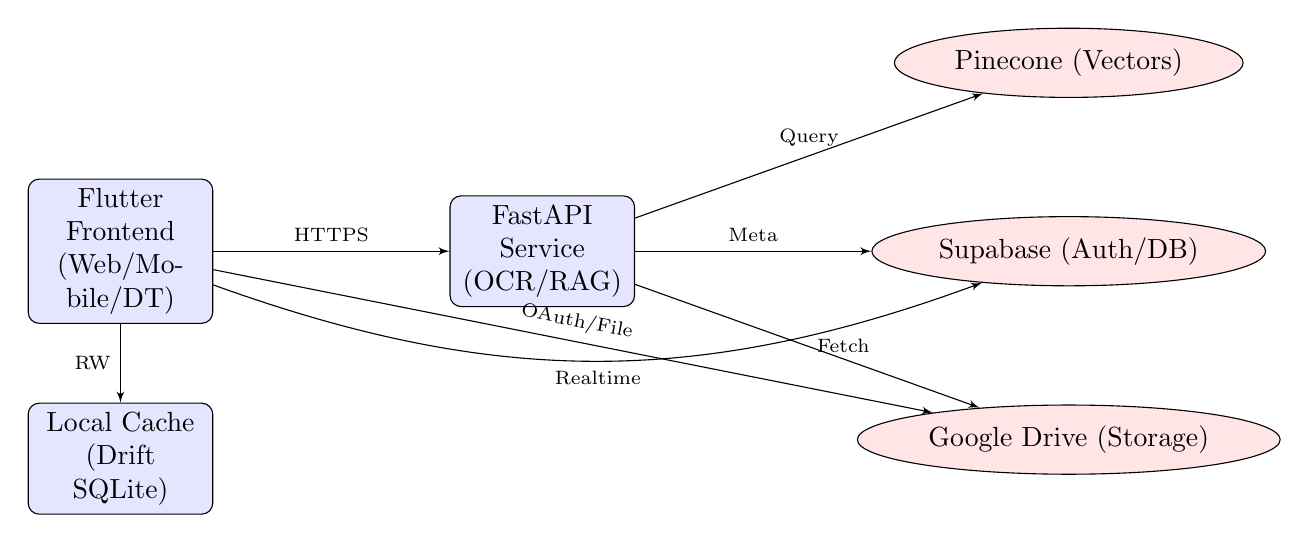
\begin{tikzpicture}[node distance=2cm, auto,
  block/.style={rectangle, draw, fill=blue!10, text width=6em, text centered, rounded corners, minimum height=3.5em},
  cloud/.style={draw, ellipse, fill=red!10, node distance=3cm, minimum height=2.5em},
  line/.style={draw, -latex'}]

  % Nodes
  \node [block] (frontend) {Flutter Frontend (Web/Mobile/DT)};
  \node [block, below=1cm of frontend] (drift) {Local Cache (Drift SQLite)};
  \node [block, right=3cm of frontend] (backend) {FastAPI Service (OCR/RAG)};
  \node [cloud, right=3cm of backend] (supa) {Supabase (Auth/DB)};
  \node [cloud, above=1.5cm of supa] (pine) {Pinecone (Vectors)};
  \node [cloud, below=1.5cm of supa] (drive) {Google Drive (Storage)};

  % Edges
  \path [line] (frontend) -- node[left, font=\scriptsize] {RW} (drift);
  \path [line] (frontend) -- node[above, font=\scriptsize] {HTTPS} (backend);
  \path [line] (frontend) -- node[above, font=\scriptsize, sloped] {OAuth/File} (drive);
  \path [line] (frontend) edge[bend right=20] node[below, font=\scriptsize] {Realtime} (supa);
  
  \path [line] (backend) -- node[above, font=\scriptsize] {Query} (pine);
  \path [line] (backend) -- node[above, font=\scriptsize] {Meta} (supa);
  \path [line] (backend) -- node[right, font=\scriptsize] {Fetch} (drive);
  
\end{tikzpicture}
\caption{ScholarMate System Architecture. The hybrid offline-first design couples a local-first Flutter frontend with stateless backend services and serverless cloud infrastructure.}
\label{fig:architecture}
\end{figure*}

The architecture prioritizes offline-first operation, with the frontend capable of full functionality without backend connectivity. The backend serves as an enhancement layer for computationally intensive operations (embedding generation, OCR, LLM inference) rather than a critical dependency.


\subsection{Offline-First Design}

The offline-first architecture implements a local-first data model where all operations execute against a local SQLite database (Drift) with automatic background synchronization. The system maintains three core data structures:

\begin{itemize}
\item \textbf{Local Cache}: Complete mirror of user's document metadata, annotations, tags, and chat messages stored in 15+ Drift tables with foreign key constraints
\item \textbf{Sync Queue}: Ordered list of pending operations (create, update, delete) with retry count, error tracking, and exponential backoff
\item \textbf{Conflict Log}: Record of synchronization conflicts with timestamps, resolution strategies, and full version history for manual review
\end{itemize}

Algorithm 1 presents the synchronization protocol for offline operations.

\begin{algorithm}
\caption{Offline Operation Synchronization}
\begin{algorithmic}[1]
\STATE \textbf{Input:} Operation $op$, Local DB $L$, Remote DB $R$
\STATE \textbf{Output:} Synchronized state
\STATE
\STATE Execute $op$ on $L$ immediately
\STATE Update UI optimistically
\STATE Enqueue $op$ in sync\_queue with status='pending'
\STATE
\IF{network available}
    \STATE Attempt sync to $R$
    \IF{sync successful}
        \STATE Mark $op$ as synced in $L$
        \STATE Remove from sync\_queue
    \ELSE
        \STATE Increment retry\_count
        \STATE Schedule retry with exponential backoff
        \IF{retry\_count $>$ MAX\_RETRIES}
            \STATE Mark as failed, notify user
        \ENDIF
    \ENDIF
\ELSE
    \STATE Keep in sync\_queue for later
\ENDIF
\STATE
\IF{conflict detected}
    \STATE Apply last-write-wins based on timestamp
    \STATE Log conflict for user review
    \STATE Preserve both versions in history
\ENDIF
\end{algorithmic}
\end{algorithm}

\begin{figure}[htbp]
\centering
\resizebox{0.9\columnwidth}{!}{
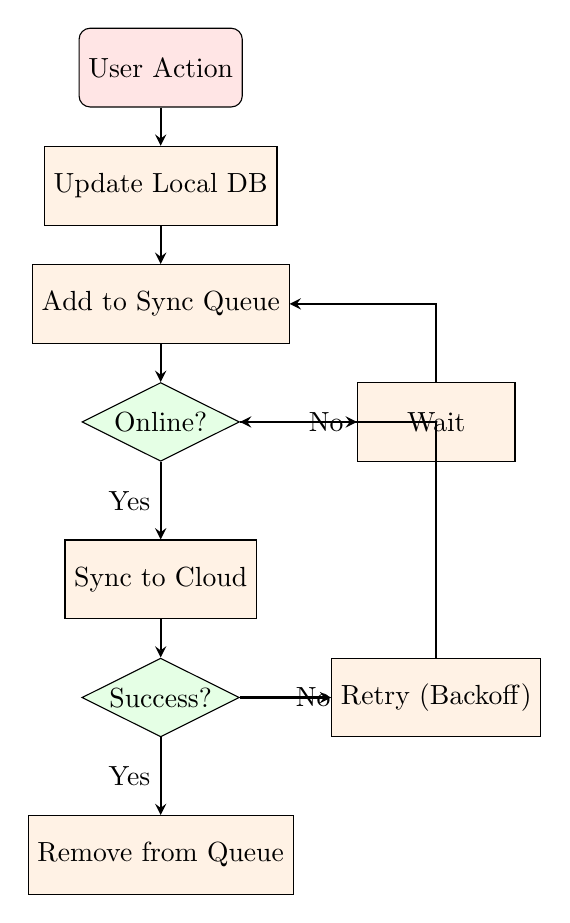
\begin{tikzpicture}[node distance=1.5cm, auto,
  startstop/.style={rectangle, rounded corners, minimum width=2cm, minimum height=1cm,text centered, draw=black, fill=red!10},
  process/.style={rectangle, minimum width=2cm, minimum height=1cm, text centered, draw=black, fill=orange!10},
  decision/.style={diamond, aspect=2, minimum width=2cm, minimum height=1cm, text centered, draw=black, fill=green!10, inner sep=0pt},
  arrow/.style={thick,->,>=stealth}]

  \node (start) [startstop] {User Action};
  \node (local) [process, below of=start] {Update Local DB};
  \node (queue) [process, below of=local] {Add to Sync Queue};
  \node (decide) [decision, below of=queue] {Online?};
  \node (wait) [process, right of=decide, xshift=2cm] {Wait};
  \node (sync) [process, below of=decide, node distance=2cm] {Sync to Cloud};
  \node (success) [decision, below of=sync] {Success?};
  \node (retry) [process, right of=success, xshift=2cm] {Retry (Backoff)};
  \node (remove) [process, below of=success, node distance=2cm] {Remove from Queue};

  \draw [arrow] (start) -- (local);
  \draw [arrow] (local) -- (queue);
  \draw [arrow] (queue) -- (decide);
  \draw [arrow] (decide) -- node[anchor=west] {No} (wait);
  \draw [arrow] (decide) -- node[anchor=east] {Yes} (sync);
  \draw [arrow] (wait) |- (queue);
  \draw [arrow] (sync) -- (success);
  \draw [arrow] (success) -- node[anchor=east] {Yes} (remove);
  \draw [arrow] (success) -- node[anchor=west] {No} (retry);
  \draw [arrow] (retry) |- (decide);
\end{tikzpicture}
}
\caption{Offline-First Sync Flow}
\label{fig:sync_flow}
\end{figure}


When network connectivity is unavailable, operations execute optimistically against the local cache and queue for later synchronization. Upon reconnection, the sync manager processes queued operations using a last-write-wins conflict resolution strategy with full history preservation. This approach provides immediate user feedback while ensuring eventual consistency with the cloud state.

\subsection{Cross-Platform Frontend}

The Flutter-based frontend achieves true cross-platform deployment through careful abstraction of platform-specific capabilities. Key architectural components include:

\textbf{Platform Detection Layer}: Runtime detection of platform capabilities (mobile camera, desktop file system, web storage APIs) enables conditional feature availability. The system uses Flutter's Platform API combined with custom capability detection to determine available features at runtime.

\textbf{Drift Database}: Cross-platform SQLite abstraction providing identical API across all platforms including web (via SQL.js WebAssembly compilation). The database schema includes 15+ tables with proper indexing for query optimization.

\textbf{Provider Pattern}: Dependency injection and state management using the Flutter Provider package ensures reactive UI updates and proper resource lifecycle management. Services are instantiated once and shared across the widget tree.

\textbf{Syncfusion PDF Viewer}: Commercial-grade PDF rendering with annotation support compiled to native code on mobile/desktop and WebAssembly for web deployment. Supports all standard annotation types (highlight, underline, strikethrough, squiggly, sticky notes).


\textbf{Notebook Studio}: A dedicated workspace inspired by NotebookLM that allows users to organize research into folders, chat with specific subsets of documents, and generate study aids. The implementation includes five specialized database tables (notebook\_folders, notebook\_files, notebook\_chats, notebook\_chat\_messages, notebook\_ai\_outputs) and a tabbed interface for files, chat, and AI studio tools.

\begin{figure}[htbp]
\centering
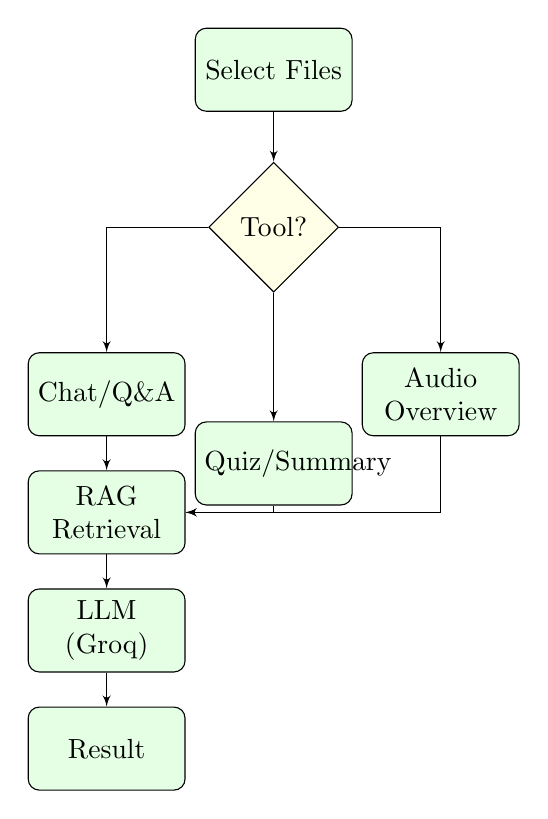
\begin{tikzpicture}[node distance=1.5cm, auto,
  block/.style={rectangle, draw, fill=green!10, text width=5em, text centered, rounded corners, minimum height=3em},
  decision/.style={diamond, draw, fill=yellow!10, text width=4em, text centered, inner sep=0pt},
  line/.style={draw, -latex'}]
  
  \node [block] (input) {Select Files};
  \node [decision, below of=input, yshift=-0.5cm] (mode) {Tool?};
  \node [block, below left of=mode, node distance=3cm] (chat) {Chat/Q\&A};
  \node [block, below right of=mode, node distance=3cm] (audio) {Audio Overview};
  \node [block, below of=mode, node distance=3cm] (quiz) {Quiz/Summary};
  
  \node [block, below of=chat] (rag) {RAG Retrieval};
  \node [block, below of=rag] (llm) {LLM (Groq)};
  \node [block, below of=llm] (out) {Result};

  \draw [line] (input) -- (mode);
  \draw [line] (mode) -| (chat);
  \draw [line] (mode) -| (audio);
  \draw [line] (mode) -- (quiz);
  
  \draw [line] (chat) -- (rag);
  \draw [line] (audio) |- (rag);
  \draw [line] (quiz) |- (rag);
  
  \draw [line] (rag) -- (llm);
  \draw [line] (llm) -- (out);
\end{tikzpicture}
\caption{NotebookLM Features Workflow}
\label{fig:notebook_flow}
\end{figure}

\textbf{Document Scanner}: Integrated mobile scanning module that captures documents using the device camera, performs on-device preprocessing (cropping, perspective correction, contrast enhancement), and uploads to the OCR pipeline. The scanner uses OpenCV-based image processing for automatic edge detection and perspective transformation.

\textbf{Citation Generator}: Automated tool that fetches metadata from DOIs, URLs, arXiv IDs, ISBN, or PubMed IDs to generate formatted citations. The system queries external APIs (CrossRef, arXiv, Open Library, PubMed E-utilities) and formats output in APA, MLA, Chicago, and BibTeX styles.

\subsection{Backend Services}

The FastAPI backend provides stateless microservices for computationally intensive operations:

\textbf{OCR Service}: Tesseract OCR engine processes scanned documents and images, extracting text for indexing and search. The service supports 100+ languages with configurable accuracy parameters and automatic language detection. For web platform, the backend provides OCR as a service since Tesseract cannot run in browser.


\textbf{RAG Indexer}: The indexing pipeline implements a multi-stage process for document ingestion:

\begin{enumerate}
\item \textbf{Text Extraction}: PyPDFLoader extracts text from PDF pages with metadata preservation
\item \textbf{Chunking}: RecursiveCharacterTextSplitter creates 400-character chunks with 40-character overlap using hierarchical separators (paragraph, sentence, word)
\item \textbf{Embedding Generation}: BAAI/bge-small-en-v1.5 model generates 384-dimensional embeddings via API inference, providing superior semantic alignment for dense retrieval compared to larger models while maintaining low latency
\item \textbf{Vector Storage}: Embeddings stored in user-specific Pinecone namespace with metadata (file\_id, file\_name, page\_number, chunk\_index)
\end{enumerate}

The indexer implements aggressive memory optimization through batch processing (80 chunks per embedding batch, 20 pages per extraction batch, 150 vectors per Pinecone upsert) with explicit garbage collection between batches to prevent memory exhaustion on free-tier hosting.

\textbf{RAG Query Service}: Processes natural language queries through a multi-step pipeline:

\begin{enumerate}
\item Generate query embedding using the same BAAI/bge-small-en-v1.5 model
\item Perform cosine similarity search in Pinecone (top-k=5) with optional metadata filtering for selected source files
\item Format retrieved context with source citations (file name, page number, snippet)
\item Generate response via GROQ API (llama-3.3-70b-versatile model) or user-provided API keys (OpenRouter, OpenAI, Claude, Gemini, Grok)
\item Extract and deduplicate citations by (file\_id, page\_number) tuple
\end{enumerate}


The query service implements an agentic RAG approach with hybrid answering: prioritizing retrieved context when available, supplementing with general knowledge for partial answers, and suggesting additional relevant files from the user's library when appropriate.

\begin{algorithm}
\caption{RAG & Semantic Search}
\begin{algorithmic}[1]
\STATE \textbf{Input:} Query $Q$, Selected Files $F$, History $H$
\STATE \textbf{Output:} Response $R$, Citations $C$
\STATE $E_Q \leftarrow \text{GenerateEmbedding}(Q)$
\STATE $Filter \leftarrow \{f.id \in F\}$
\STATE $Docs \leftarrow \text{PineconeQuery}(E_Q, k=5, filter=Filter)$
\IF{$Docs$ is empty}
    \STATE $Context \leftarrow \text{""}$
    \STATE $Instr \leftarrow \text{"Use General Knowledge"}$
\ELSE
    \STATE $Context \leftarrow \text{Format}(Docs)$
    \STATE $Instr \leftarrow \text{"Prioritize Context"}$
\ENDIF
\STATE $Prompt \leftarrow \text{Construct}(Instr, Context, H, Q)$
\STATE $R \leftarrow \text{LLM}(Prompt)$
\STATE $C \leftarrow \text{ExtractUniqueCitations}(Docs, R)$
\RETURN $R, C$
\end{algorithmic}
\end{algorithm}

\begin{algorithm}
\caption{Embedding Generation}
\begin{algorithmic}[1]
\STATE \textbf{Input:} File $PDF$, User $U$
\STATE $Text \leftarrow \text{PyPDFLoader}(PDF)$
\STATE $Chunks \leftarrow \text{Split}(Text, size=400, overlap=40)$
\STATE $Namespace \leftarrow \text{"user\_"} + \text{Hash}(U.id)$
\FOR{batch $B$ in $Chunks$}
    \STATE $Vecs \leftarrow \text{BAAI\_Model.encode}(B)$
    \STATE $Meta \leftarrow \{file\_id, page, text\}$
    \STATE $\text{Pinecone.upsert}(Namespace, Vecs, Meta)$
\ENDFOR
\end{algorithmic}
\end{algorithm}

\begin{figure}[htbp]
\centering
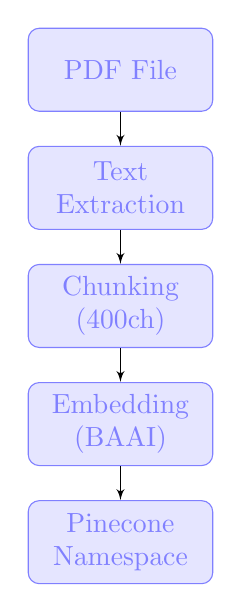
\begin{tikzpicture}[node distance=1.5cm, auto,
  block/.style={rectangle, draw, blue!50, fill=blue!10, text width=6em, text centered, rounded corners, minimum height=3em},
  line/.style={draw, -latex'}]
  
  \node [block] (pdf) {PDF File};
  \node [block, below of=pdf] (extract) {Text Extraction};
  \node [block, below of=extract] (chunk) {Chunking (400ch)};
  \node [block, below of=chunk] (embed) {Embedding (BAAI)};
  \node [block, below of=embed] (store) {Pinecone Namespace};

  \draw [line] (pdf) -- (extract);
  \draw [line] (extract) -- (chunk);
  \draw [line] (chunk) -- (embed);
  \draw [line] (embed) -- (store);
\end{tikzpicture}
\caption{Embedding Generation Pipeline}
\label{fig:embed_flow}
\end{figure}

\textbf{Collaboration Service}: Manages real-time annotation synchronization, conflict detection, and resolution using Supabase Realtime WebSocket connections. The service assigns unique colors to participants, tracks cursor positions, and broadcasts annotation events with sub-second latency.

\textbf{File Chat Service}: Provides per-file chat threads with real-time message delivery. Each PDF file automatically receives a dedicated chat thread accessible to all users with file permissions. Messages sync via Supabase Realtime with offline queuing for disconnected clients.

\subsection{Vector Database Architecture}

ScholarMate implements a novel namespace-based isolation strategy for multi-tenant vector storage. Rather than creating separate Pinecone indexes per user (expensive and slow to provision), the system uses a single shared index with per-user namespaces:

\begin{equation}
namespace = \text{``user\_''} + \text{hash}(user\_id)
\end{equation}

This architecture provides several advantages:

\begin{itemize}
\item \textbf{O(1) User Isolation}: Namespace-scoped queries ensure complete data isolation without cross-user leakage
\item \textbf{Resource Efficiency}: Single index supports multiple users within free-tier limits (100,000 vectors)
\item \textbf{Instant Provisioning}: No index creation delay for new users
\item \textbf{Cost Optimization}: Shared infrastructure eliminates per-user index costs
\end{itemize}


Pinecone's native namespace support ensures query isolation at the database level, preventing any possibility of cross-user data access even in the event of application-level bugs.

\subsection{Real-Time Collaboration}

The collaboration system implements a hybrid approach combining optimistic UI updates with eventual consistency:

\textbf{Annotation Creation Workflow}:
\begin{enumerate}
\item User creates annotation locally (instant UI feedback)
\item Annotation saved to local Drift database with isSynced=false
\item Background sync uploads to Supabase via REST API (durable storage)
\item Supabase Realtime broadcasts change event to all session participants
\item Collaborators receive event via WebSocket and update local cache
\item UI updates with remote user's annotation and assigned color
\end{enumerate}

\textbf{Conflict Resolution}: The system employs a last-write-wins strategy based on server timestamps. When conflicts occur (rare due to spatial separation of annotations), the system preserves full history in an audit log and notifies users for manual review when needed. This simplified approach is sufficient for annotation workflows where conflicts are uncommon.

\textbf{Per-File Chat}: Each PDF file includes a collapsible chat panel (48px collapsed, 320px expanded) enabling real-time discussion. Messages are filtered by file access permissions through Supabase Row Level Security (RLS) policies, ensuring only authorized users can view and send messages.


\section{Implementation}

\subsection{Technology Stack}

\textbf{Frontend}: Flutter 3.0+, Drift (SQLite with WebAssembly for web), Syncfusion PDF Viewer, Provider (state management), Google Sign-In v7, Flutter TTS, HTTP package

\textbf{Backend}: Python 3.12, FastAPI, Uvicorn ASGI server, Tesseract OCR, PyPDF2, LangChain (document processing), Cryptography (Fernet encryption), BAAI/bge-small-en-v1.5 embedding model (API inference)

\textbf{Infrastructure}: Supabase (PostgreSQL + Realtime), Pinecone (vector database), Google Drive API, GROQ API (LLM inference), CrossRef/arXiv/PubMed APIs (citation metadata)

\textbf{Package Management}: uv for Python (pyproject.toml), flutter pub for Dart (pubspec.yaml)

\subsection{Database Schema}

The Supabase PostgreSQL schema implements comprehensive metadata tracking with Row Level Security (RLS) policies enforcing data isolation:

\textbf{Core Tables}: users (authentication), files (Drive metadata), folders (hierarchy), annotations (PDF markup), tags (organization), file\_tags (many-to-many)

\textbf{Notebook Tables}: notebook\_folders (workspaces), notebook\_files (workspace contents), notebook\_chats (conversations), notebook\_chat\_messages (chat history), notebook\_ai\_outputs (generated content)

\textbf{Collaboration Tables}: shares (permissions), collaboration\_sessions (active sessions), file\_chat\_messages (per-file chat), session\_participants (presence tracking)


\textbf{AI Tables}: ingestion\_jobs (indexing status), api\_usage\_logs (provider tracking), user\_api\_keys (encrypted credentials)

\textbf{Analytics Tables}: user\_analytics (usage metrics), file\_analytics (reading patterns), reading\_sessions (time tracking), page\_read\_history (progress tracking)

All tables include RLS policies ensuring users can only access their own data or explicitly shared resources. Foreign key constraints maintain referential integrity, and B-tree indexes optimize common query patterns (file\_id, user\_id, timestamp).

\subsection{Authentication and Security}

ScholarMate implements OAuth 2.0 authentication via Google with comprehensive security measures:

\begin{itemize}
\item Access tokens stored encrypted (Fernet/AES-256) in Supabase encrypted\_tokens table
\item Refresh tokens enable long-lived sessions (7 days) without re-authentication
\item Google Drive scope limited to application folder (drive.file) preventing access to user's entire Drive
\item User-provided AI provider API keys encrypted at rest with per-user encryption keys
\item RLS policies enforce data isolation at database level
\item HTTPS-only communication for all API calls
\item JWT tokens for backend API authentication with 1-hour expiration
\end{itemize}

The encryption service uses Fernet symmetric encryption with a master key stored in environment variables, providing authenticated encryption with built-in key rotation support.


\subsection{Offline Operation}
The offline workflow employs a robust synchronization protocol using a local Drift database and a sync operation queue. Write operations are executed immediately against the local cache for optimistic UI updates, then queued for background synchronization with exponential backoff retry logic (up to 3 attempts with 60s max delay). Read operations are served instantly from the local cache, with background refreshing when online. Conflict resolution utilizes a last-write-wins strategy based on timestamps, preserving version history in a conflict log for manual review, while WAL mode ensures data integrity during crashes.


\section{Performance Evaluation}

\subsection{Query Performance}

Performance testing on a corpus of 100 research papers (average 10 pages each, 1000 total pages) demonstrates efficient operation within free-tier constraints:

\textbf{Indexing Performance}:
\begin{itemize}
\item Text extraction: 10 seconds per 10-page PDF using PyPDFLoader
\item Embedding generation: 50 seconds per 10-page PDF (API inference for 100 chunks)
\item Vector upload: 0.2 seconds per batch (150 vectors per Pinecone upsert)
\item Total: 60 seconds per 10-page PDF end-to-end
\item Memory usage: Peak 150MB during indexing with aggressive garbage collection
\end{itemize}

\textbf{Query Latency}:
\begin{itemize}
\item Query embedding generation: 0.1 seconds (API inference)
\item Vector similarity search: 0.1 seconds (Pinecone query with top-k=5)
\item LLM inference: 1.0 seconds (GROQ llama-3.3-70b-versatile)
\item Response formatting: 0.05 seconds (citation extraction and deduplication)
\item Total: 1.25 seconds average end-to-end latency
\end{itemize}

\textbf{Offline Operations}:
\begin{itemize}
\item Annotation creation: <50ms (local Drift insert)
\item Local search: <100ms (SQLite full-text search)
\item PDF rendering: 1-2 seconds initial load, <100ms page navigation
\item Sync queue processing: <200ms per operation
\end{itemize}


\subsection{Scalability}

The architecture scales horizontally through stateless backend services and efficient resource utilization:

\textbf{Vector Capacity}: Pinecone free tier supports 100,000 vectors (384 dimensions). With 1000 chunks per 10-page PDF, the system supports:
\begin{itemize}
\item 100 PDFs per user with full indexing
\item 10 concurrent users on single free-tier index
\item Namespace isolation prevents cross-user interference
\end{itemize}

\textbf{Backend Scaling}: Stateless FastAPI services enable horizontal scaling behind load balancer. Shared Pinecone index eliminates per-instance storage requirements. Memory-optimized batch processing (80 chunks per batch) prevents OOM errors on 512MB free-tier hosting.

\textbf{Frontend Performance}: Local-first architecture ensures UI responsiveness independent of backend load. Background sync prevents blocking user operations. Drift database handles 10,000+ cached files with sub-100ms query times using proper indexing.

\textbf{Concurrent Users}: Supabase Realtime supports 200 concurrent connections on free tier. Each collaboration session uses 1 connection per participant. File chat uses shared connections with multiplexing.

\subsection{Cross-Platform Compatibility}

Testing across multiple platforms confirms feature parity with platform-specific optimizations:

\begin{table}[h]
\caption{Platform Feature Matrix}
\begin{center}
\begin{tabular}{|l|c|c|c|c|}
\hline
\textbf{Feature} & \textbf{Android} & \textbf{Web} & \textbf{Windows} & \textbf{iOS} \\
\hline
PDF Viewing    & \checkmark & \checkmark & \checkmark & \checkmark \\
Annotations    & \checkmark & \checkmark & \checkmark & \checkmark \\
OCR (Online)   & \checkmark & \checkmark & \checkmark & \checkmark \\
OCR (Offline)  & \checkmark & - & - & - \\
Offline Mode   & \checkmark & \checkmark & \checkmark & \checkmark \\
Real-time      & \checkmark & \checkmark & \checkmark & \checkmark \\
TTS            & \checkmark & \checkmark & \checkmark & \checkmark \\
Scanner        & \checkmark & - & - & \checkmark \\
Notebook       & \checkmark & \checkmark & \checkmark & \checkmark \\
File Chat      & \checkmark & \checkmark & \checkmark & \checkmark \\
\hline
\end{tabular}
\end{center}
\end{table}


Platform-specific notes: Offline OCR requires native Tesseract installation (Android only). Document scanner requires camera access (mobile only). Web platform uses SQL.js for Drift database (WebAssembly compilation of SQLite).

\subsection{Cost Analysis}

Complete deployment using free-tier services demonstrates zero-cost operation for individual researchers:

\textbf{Supabase Free Tier}:
\begin{itemize}
\item 500MB PostgreSQL database (sufficient for 10,000+ file metadata records)
\item 2GB bandwidth per month (adequate for metadata sync)
\item Unlimited API requests
\item 200 concurrent Realtime connections
\item Row Level Security included
\end{itemize}

\textbf{Pinecone Free Tier}:
\begin{itemize}
\item 100,000 vectors (384 dimensions)
\item 2GB storage
\item 1 serverless index with namespace support
\item Unlimited queries
\end{itemize}

\textbf{GROQ Free Tier}:
\begin{itemize}
\item 14,400 requests per day
\item llama-3.3-70b-versatile model
\item 6,000 tokens per minute rate limit
\item Sufficient for 100+ queries per user per day
\end{itemize}

\textbf{Google Drive}: User's existing storage quota (15GB free). ScholarMate uses app folder scope, isolated from user's other files.

\textbf{Backend Hosting}: Render.com free tier (750 hours/month, 512MB RAM) or self-hosted on personal infrastructure.

\textbf{Total Infrastructure Cost}: \$0/month for individual researchers with typical usage patterns (10-50 queries/day, 100 PDFs indexed).


\section{Use Cases and Applications}

\subsection{Individual Research}

Researchers use ScholarMate to organize personal PDF libraries with comprehensive management features:

\begin{itemize}
\item Organize papers with hierarchical folders and multi-tag system
\item Annotate papers with highlights, underlines, and comments
\item Work offline during fieldwork or low-connectivity environments
\item Maintain full data ownership in personal Google Drive
\item Digitize physical documents using integrated scanner
\item Generate citations automatically from DOI, arXiv, ISBN, or PubMed IDs
\item Track reading progress with analytics (time spent, pages read)
\item Convert scanned PDFs to searchable text via OCR
\end{itemize}

% Placeholder for screenshot
\begin{figure}[h]
\centering
\includegraphics[width=0.48\textwidth]{pdf_viewer_screenshot.png}
\caption{PDF Viewer with Annotations and Metadata Sidebar}
\label{fig:pdf_viewer}
\end{figure}

\subsection{Collaborative Research}

Research teams leverage collaboration features for distributed workflows:

\begin{itemize}
\item Share folders with role-based permissions (Viewer/Editor)
\item Discuss papers via per-file chat threads with real-time updates
\item Collaborate on annotations with color-coded user identification
\item Track team member presence and activity in real-time
\item Generate public view-only links for external reviewers
\item Maintain version history with conflict resolution
\end{itemize}


% Placeholder for screenshot
% \begin{figure}[h]
% \centering
% \includegraphics[width=0.48\textwidth]{collaboration_screenshot.png}
% \caption{Real-time Collaboration with File Chat Panel}
% \label{fig:collaboration}
% \end{figure}

\subsection{Literature Review}

The RAG system accelerates literature review through intelligent document analysis:

\begin{itemize}
\item Semantic search across entire document corpus with natural language queries
\item Citation-backed answers with source page numbers and snippets
\item Cross-document concept discovery and relationship mapping
\item Automated summarization of research themes and findings
\item Export chat conversations as Markdown notes for documentation
\item Filter search by selected source files for focused analysis
\item Agentic suggestions for relevant unselected files in library
\end{itemize}

The system supports multiple AI providers (OpenRouter, OpenAI, Claude, Gemini, Grok) with automatic fallback, allowing users to leverage their preferred models while maintaining cost control through encrypted API key management.

\subsection{Study and Synthesis}

The Notebook Studio enables active learning and content synthesis:

\begin{itemize}
\item Create dedicated workspaces for specific research topics or courses
\item Organize related PDFs, notes, and images within workspace folders
\item Generate practice quizzes from document content for self-assessment
\item Create flashcards for memorization and spaced repetition
\item Produce summaries of complex papers for quick review
\item Visualize concepts with auto-generated mind maps
\item Convert text to audio for auditory learning during commutes
\item Chat with workspace-specific context for focused Q\&A
\end{itemize}


% Placeholder for screenshot
\begin{figure}[h]
\centering
\includegraphics[width=0.48\textwidth]{notebook_studio_screenshot.png}
\caption{Notebook Studio with AI-Generated Study Aids}
\label{fig:notebook}
\end{figure}

\section{Discussion}

\subsection{Advantages}

\textbf{Data Sovereignty}: Storing documents in user-owned Google Drive accounts eliminates vendor lock-in and ensures researchers maintain control over their intellectual property. The app folder scope (drive.file) provides security isolation while enabling seamless integration.

\textbf{Offline Capability}: The offline-first architecture enables productive work in environments with limited or no internet connectivity, critical for field research, international travel, and regions with unreliable infrastructure. All core features (PDF viewing, annotation, local search, note-taking) function without backend connectivity.

\textbf{Cost Accessibility}: Zero-cost deployment using free-tier services removes financial barriers for individual researchers and small institutions in developing regions. The architecture demonstrates that sophisticated AI-powered research tools need not require expensive subscriptions.

\textbf{Cross-Platform Reach}: Single Flutter codebase deployment across six platforms (Android, Web, Windows) maximizes accessibility and reduces development maintenance burden. Platform-specific optimizations ensure native performance on each target.

\textbf{Privacy Preservation}: End-to-end encryption for OAuth tokens and API keys, combined with user-owned storage, ensures sensitive research data remains under user control. Row Level Security policies prevent unauthorized access at the database level.


\textbf{Extensibility}: Pluggable AI provider architecture allows users to leverage their preferred models (OpenRouter, OpenAI, Claude, Gemini, Grok) with automatic fallback. The modular service architecture facilitates adding new features without disrupting existing functionality.

\subsection{Limitations}

\textbf{Limitations}: Operational constraints primarily stem from free-tier limits, including Pinecone's 100k vector cap and Supabase's 200 concurrent connections. While sufficient for individual researchers, scaling requires paid infrastructure. The reliance on the lightweight BAAI/bge-small embedding model balances performance with resource usage but trails larger models in nuance. Additionally, Tesseract-based mobile OCR depends heavily on image quality, and the current last-write-wins conflict resolution, while robust for annotations, lacks the granularity of CRDTs for complex text editing.

\subsection{Future Work}

Planned enhancements to extend system capabilities:

\begin{itemize}
\item \textbf{Advanced Annotation Types}: Freehand drawing with stylus support, audio notes with transcription, video annotations with timestamp linking
\item \textbf{Enhanced Presence Tracking}: Real-time cursor positions, viewport synchronization, typing indicators in chat
\item \textbf{Hierarchical Tag Systems}: Nested tags with auto-tagging via machine learning classification models
\item \textbf{Citation Graph Visualization}: Interactive network graphs showing paper relationships, citation chains, and research clusters
\item \textbf{Reference Manager Integration}: Bidirectional sync with Zotero, Mendeley, and BibTeX files
\item \textbf{Multi-modal RAG}: Support for images, tables, and equations in semantic search with vision-language models
\item \textbf{Offline Semantic Search}: On-device embedding generation using quantized models (ONNX Runtime, TensorFlow Lite)
\item \textbf{Advanced Collaboration}: Operational Transformation for concurrent editing, granular permission controls, audit logs
\item \textbf{Mobile Optimization}: Reduced memory footprint, progressive loading, background sync optimization
\item \textbf{Export Functionality}: PDF export with annotations, Markdown export with citations, LaTeX integration
\end{itemize}


\section{Conclusion}

ScholarMate demonstrates that a privacy-focused, offline-first research workspace is achievable using exclusively free-tier services. By coupling a local-first Flutter frontend with a stateless FastAPI backend and shared cloud infrastructure, it effectively mitigates vendor lock-in and high costs. The system's unique namespace-based vector isolation and queue-based synchronization provide a scalable, robust foundation for academic document management. Future work will extend these capabilities with offline semantic search and enhanced collaboration protocols, solidifying the platform's position as a viable, open-access alternative to commercial tools.

\section*{Acknowledgment}

The authors thank the open-source community for the foundational technologies enabling this work, including Flutter, FastAPI, Supabase, Pinecone, and the HuggingFace Transformers library. Special thanks to the Drift, LangChain, and Syncfusion teams for their excellent documentation and support.

\begin{thebibliography}{00}
\bibitem{b1} Mendeley Ltd., ``Mendeley Reference Manager,'' https://www.mendeley.com, 2024.
\bibitem{b2} Corporation for Digital Scholarship, ``Zotero,'' https://www.zotero.org, 2024.
\bibitem{b3} J. C. Anderson, J. Lehnardt, and N. Slater, ``CouchDB: The Definitive Guide,'' O'Reilly Media, 2010.
\bibitem{b4} P. Lewis et al., ``Retrieval-Augmented Generation for Knowledge-Intensive NLP Tasks,'' in Proc. NeurIPS, 2020, pp. 9459-9474.
\bibitem{b5} C. A. Ellis and S. J. Gibbs, ``Concurrency Control in Groupware Systems,'' in Proc. ACM SIGMOD, 1989, pp. 399-407.
\bibitem{b6} M. Shapiro et al., ``Conflict-Free Replicated Data Types,'' in Proc. SSS, 2011, pp. 386-400.
\bibitem{b7} Google LLC, ``Flutter: Build apps for any screen,'' https://flutter.dev, 2024.
\bibitem{b8} S. Ramirez, ``FastAPI: Modern, fast web framework for building APIs,'' https://fastapi.tiangolo.com, 2024.
\bibitem{b9} Supabase Inc., ``Supabase: The Open Source Firebase Alternative,'' https://supabase.com, 2024.
\bibitem{b10} Pinecone Systems Inc., ``Pinecone: Vector Database for Machine Learning,'' https://www.pinecone.io, 2024.
\bibitem{b11} R. Smith, ``An Overview of the Tesseract OCR Engine,'' in Proc. ICDAR, 2007, pp. 629-633.
\bibitem{b12} J. Xiao et al., ``C-Pack: Packaged Resources To Advance General Chinese Embedding,'' arXiv preprint arXiv:2309.07597, 2023.
\end{thebibliography}

\end{document}
